% The Clever Algorithms Project: http://www.CleverAlgorithms.com
% (c) Copyright 2011 Jason Brownlee. Some Rights Reserved. 
% This work is licensed under a Creative Commons Attribution-Noncommercial-Share Alike 2.5 Australia License.

% Name
% The algorithm name defines the canonical name used to refer to the technique, in addition to common aliases, abbreviations, and acronyms. The name is used in terms of the heading and sub-headings of an algorithm description.
\section{Conjugate Gradient Method} 
\label{sec:conjugate_gradient}
\index{Conjugate Gradient Method}
\index{Nonlinear Conjugate Gradient Method}

% other names
% What is the canonical name and common aliases for a technique?
% What are the common abbreviations and acronyms for a technique?
\emph{Conjugate Gradient Method, Nonlinear Conjugate Gradient Method.}

% Taxonomy: Lineage and locality
\subsection{Taxonomy}
% To what fields of study does a technique belong?
Conjugate Gradient Method is a first-order derivative optimization method for multidimensional nonlinear unconstrained functions.
% What are the closely related approaches to a technique?
It is related to other first-order derivative optimization algorithms such as Gradient Descent and Steepest Descent.

% Strategy: Problem solving plan
% The strategy is an abstract description of the computational model. The strategy describes the information processing actions a technique shall take in order to achieve an objective. The strategy provides a logical separation between a computational realization (procedure) and a analogous system (metaphor). A given problem solving strategy may be realized as one of a number specific algorithms or problem solving systems. The strategy description is textual using information processing and algorithmic terminology.
\subsection{Strategy}
% What is the information processing objective of a technique?
The information processing objective of the technique is to locate the extremum of a function.
% What is a techniques plan of action?
From a starting position, the method first computes the gradient to locate the direction of steepest descent, then performs a line search to locate the optimum step size ($\alpha$). The method then repeats the process of computing the steepest direction, computes direction of the search, and performing a line search to locate the optimum step size. A parameter $\beta$ defines the direction update rule based on the gradient and can be computed using one of a number of methods.
% difference from steepest descent
The difference between Conjugate Gradient and Steepest Descent is that it uses conjugate directions rather than local gradients to move downhill towards the function minimum, which can be very efficient.

% Heuristics: Usage guidelines
% The heuristics element describe the commonsense, best practice, and demonstrated rules for applying and configuring a parameterized algorithm. The heuristics relate to the technical details of the techniques procedure and data structures for general classes of application (neither specific implementations not specific problem instances). The heuristics are described textually, such as a series of guidelines in a bullet-point structure.
\subsection{Heuristics}
% What are the suggested configurations for a technique?
% What are the guidelines for the application of a technique to a problem instance?

\begin{itemize}
	\item It is more efficient than Steepest Descent, for example it may take a straight line path down narrow valley's, whereas Steepest Descent would have to zig-zag (pinball) down the valley.
	\item Devolves into Steepest Descent if the conjugate direction is reset each iteration.
	\item It is almost as fast as second-order gradient methods, requiring just $n$ iterations to locate an optimum for suitable functions (where $n$ is the number of parameters).
	\item It does not maintain a Hessian matrix (like BFGS) and therefore may be suitable for larger problems with many variables.
	\item The method is most efficient (works the best) with quadratic or quadratic-like functions, or where the function is approximately quadratic near the optimum.
	\item The method is sensitive to its starting position on non-convex problems.
	\item The learning rate (step size $\alpha$) does not have to be specified as a line search is used to locate the optimum value as needed.
	\item Common methods for computing the direction update rule ($\beta$) are the Hestenes-Stiefel \cite{Hestenes1952}, Fletcher-Reeves \cite{Fletcher1964}, Polak-Ribi\`ere \cite{Polak1969} (French), and Beale-Sorenson \cite{Beale1972, Sorenson1969} methods. The Polak-Ribi\`ere method generally works better in practice for non-quadratic functions.
	\item It is dependent on the accuracy of the line search, errors introduced both from this and the less-than quadratic nature of the response surface will result in more frequent updates to the direction and a less efficient search.
	\item To avoid the search degenerating, consider restarting the search process after $n$ iterations, where $n$ is the number of function parameters.
\end{itemize}


% sample script in R
\subsection{Code Listing}
% listing
Listing~\ref{stats_conjugate_gradient} provides a code listing of the Conjugate Gradient method in R solving a two-dimensional nonlinear optimization function. Figure~\ref{plot:conjugate_gradient_result} provides a plot of the test problem with the located minimum highlighted.

% algorithm and package
The example uses the \texttt{optim()} function in the \texttt{stats} core package configured to use the Conjugate Gradient Method as ``CG'' \cite{RDCT2011a}. The method supports three update methods: Fletcher-Reeves update (default), Polak-Ribi\`ere update, and the Beale-Sorenson update. The \texttt{optim} function is for General-purpose Optimization, for more information on this library type: \texttt{library(help="stats")}, and for more information on the function type: \texttt{?optim}.

% problem
The test problem is the Rosenbrock function in two-dimensions where the optimum is at $x,y=1$. The starting position for the algorithm is taken as a random point $x,y \in [-3,3]$. The gradient for this function is specified and is used by the optimization method.

\lstinputlisting[firstline=7,language=r,caption={Example of Conjugate Gradient in R using the \texttt{optim()} function in the \texttt{stats} core package.}, label=stats_conjugate_gradient]{../src/algorithms/optimization/stats_conjugate_gradient.R}

\begin{figure}[htp]
\centering
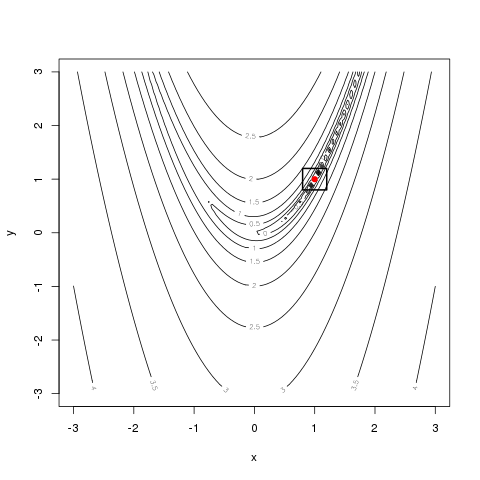
\includegraphics[scale=0.45]{a_optimization/conjugate_gradient_result.png}
\caption{Contour plot of the Rosenbrock function with the located minimum highlighted.}
\label{plot:conjugate_gradient_result}
\end{figure}

% other packages
The \texttt{gsl} package in the \texttt{multimin()} function provides an implementation of Conjugate Gradient Method that makes use of the GNU Scientific Library \cite{Hankin2011}.


% References: Deeper understanding
% The references element description includes a listing of both primary sources of information about the technique as well as useful introductory sources for novices to gain a deeper understanding of the theory and application of the technique. The description consists of hand-selected reference material including books, peer reviewed conference papers, journal articles, and potentially websites. A bullet-pointed structure is suggested.
\subsection{References}
% What are the primary sources for a technique?
% What are the suggested reference sources for learning more about a technique?

% primary sources
\subsubsection{Primary Sources}
% seminal
The Conjugate Gradient method for solving systems of linear equations was proposed by Hestenes and Stiefel in 1952 \cite{Hestenes1952}.
% optimization
Fletcher and Reeves extended the method to an optimization method for unconstrained nonlinear optimization in 1964 \cite{Fletcher1964}.

% more info
\subsubsection{More Information}
% book
Polak provides a detailed treatment of Conjugate Gradient in his text of numerical methods with suggested implementation details \cite{Polak1971} (pages 44 and 306).
Hestenes also provides a treatment of Conjugate Gradient and other numerical methods for optimization in his text \cite{Hestenes1980}.
Fletcher also wrote a book on numerical analysis for optimization with a clear treatment of Conjugate Direction Methods including Conjugate Gradient \cite{Fletcher2000} (chapter 4).
% review paper
Shewchuk provides a detailed treatment of the method and usage considerations \cite{Shewchuk1994} (page 42).
% implementation details
Press et~al.\ provide a good summary of the method with sample code in the C programming language \cite{Press2007}.

% END
